\documentclass{sig-alternate}%[conference][letterpaper]
\usepackage{times,epsfig,proof,url,algorithm,bm}
\usepackage[noend]{algpseudocode}
\usepackage{amsmath}
\usepackage{textcomp}
\usepackage{graphicx}
\usepackage{subfigure}
\usepackage{multirow}
\usepackage{color}
%\newcommand{\tab}{\hspace*{2ex}}
%\newcommand{\shrink}{\vspace*{-2ex}}
%\newcommand{\cut}[1]{}

\newtheorem{newproperty}{Property}
\newtheorem{newrule}{Rule}
\newtheorem{theorem}{Theorem}[section]
\newtheorem{lemma}[theorem]{Lemma}
\newcommand{\figref}[1]{Figure \ref{#1}}
\newcommand{\tabref}[1]{Table \ref{#1}}
\newcommand{\secref}[1]{Section \ref{#1}}
\newcommand{\algoref}[1]{Algorithm \ref{#1}}
\newcommand{\I}{\mathcal{I}}
\newcommand{\LEN}{\mathcal{L}}
\newcommand{\R}{\mathcal{R}}
\newcommand{\T}{\mathcal{T}}
\newcommand{\D}{\mathcal{D}}
\newcommand{\M}{\mathcal{M}}
\renewcommand{\algorithmicrequire}{\textbf{Input:}}
\renewcommand{\algorithmicensure}{\textbf{Output:}}
\newcommand{\KZ}[1]{\textcolor{blue}{[KZ: #1]}}
\newcommand{\JK}[1]{\textcolor{red}{[JK: #1]}}
\begin{document}
\conferenceinfo{IH\&MMSec'13,} {June 17--19, 2013, Montpellier, France.} 
\CopyrightYear{2013} 
\crdata{978-1-4503-2081-8/13/06}
\clubpenalty=10000 
\widowpenalty = 10000
\title{Watermarking Road Maps against
Crop and Merge Attacks}

\numberofauthors{4}
\author{
\alignauthor
Kai Jiang\hspace*{3mm} Kenny Q. Zhu\\
       \affaddr{Shanghai Jiao Tong University}\\
       \affaddr{Shanghai, China}\\
       \email{jkai@sjtu.edu.cn, kzhu@cs.sjtu.edu.cn}
\alignauthor
Yan Huang \\
       \affaddr{University of North Texas}\\
       \affaddr{Denton, TX, USA}\\
       \email{huangyan@unt.edu}
\alignauthor 
Xiaobin Ma \\
       \affaddr{1 Oracle Drive}\\
       \affaddr{Nashua, NH, USA}\\
       \email{xiaobin@cs.umn.edu}
}

%
%\author{
%\alignauthor
%Kai Jiang\\
%       \affaddr{Shanghai Jiao Tong University}\\
%       \affaddr{Shanghai, China}\\
%       \email{jkai@sjtu.edu.cn}
%\alignauthor
%Kenny Q. Zhu \\
%       \affaddr{Shanghai Jiao Tong University}\\
%       \affaddr{Shanghai, China}\\
%       \email{kzhu@cs.sjtu.edu.cn}
%\alignauthor
%Yan Huang \\
%       \affaddr{University of North Texas}\\
%       \affaddr{Denton, TX, USA}\\
%       \email{huangyan@unt.edu}
%\alignauthor
%Xiaobin Ma \\
%       \affaddr{University of North Texas}\\
%       \affaddr{Denton, TX, USA}\\
%       \email{xiaobin@unt.edu}
%}
\maketitle

\begin{abstract}

%Protecting the copyrights of intelligent electric products is an urgent task around the world. One way to deter piracy
%of these products is to make illegal copying very difficult or impossible by approaches such as encryption. A complimentary 
%approach is to embed digital watermarks into the electric products.
%Digital road maps are a valuable resource for GPS navigation and other GIS applications. 
%It is a form of vector graphics but with spatial-geometric properties.
%Watermarking is an important mechanism to protect the copyright of digital
%road maps.  
Past research on watermarking digital road maps has been focused on
deterring common attacks such as adding noise to the whole map so as to
destroy the embedded watermarks. This paper focuses on two less common but
increasingly used types of attack: crop attacks and merge attacks. 
Crop attack crops a fragment of the original map and uses the fragment as a new
map. When the new map is much smaller than the original map, it is called
massive cropping. Merge attack merges maps from various sources together
to form a new map. 
Conventional watermarking techniques fail against these attacks
either because they require global information from the whole map or
they must add too many local watermarks and affect the usability of the maps.
%these two types of attacks totally because they detect waterwarks based on
%global information from the whole map, or they must divide the map into many small
%segments and add many more watermarks locally and thus affect the perception
%and usability of the maps. 
This paper proposes a novel quad-tree based
blind watermarking scheme that partitions the original map according to
the quad-tree and plants just one single bit in each sub-region of the
map. The approach achieves almost 100\% detection accuracy for moderate
crop and merge attacks, and over 80\% accuracy with more than 95\% of the 
original map cropped and removed. Furthermore, the method introduces 
very little distortion to the original map: 
to effectively protect a 23.5MB Minneapolis-St.Paul map against
crop and merge as well as other common attacks, only
423 bits or 53 bytes of watermark is required.
\footnote{Kenny Q. Zhu (the corresponding author) is partially supported 
by NSFC grants 61033002 and 61100050.}
% 
%
%
%
%In this research, we analyse the properties of digital road maps and propose
%a novel blind watermarking framework to protect the IP rights of owners of
%the maps.
%The framework makes use of local information which is collected by a 
%modified Quadtree structure and inserts watermarks according to the density of
%the map. The framework also allows the detection of the illegal use of a
%watermarked map without reference to the original map at all.
%The most important advantage of this framework is that it detects illegal
%use of even a small part of a protected map, in what we call ``massive crop attacks'' 
%and ``merge attacks'', which were previously unsolved problems. 
%The evaluation shows that our approach offers high accuracy with very reasonable
%time complexity.
%
%\KZ{Key points: Traditional watermarking techniques don't handle cropping and
%merging attacks well and they incur bigger distortion to the maps. We are 1) blind;
%2) light-weight (nlogn); 3) limited distortion (only a number of bits are changed);
%4) localized watermarks that can handle massive cropping and merging attacks.}
\end{abstract}
\category{D.2.11}{Software Architectures}{Information hiding} 
\category{D.4.6}{Security and Protection}{Authentication}
\keywords{Watermark, digital road map, quad-tree, crop attack, merge attack}

\section{Introduction}

Protein$-$protein interactions (PPIs) are of central importance for the majority of biological functions, such as signal transduction, metabolic pathways, molecular dynamics, and protein networks\cite{Hoffmann.Krallinger.ea:2005}, for they serve as the most fundamental building blocks of the entire interacademic systems of any organisms. Collecting data on pairwise interaction relationships is essential for multiple purpose, including identification of modules with certain functionality\cite{Spirin.Mirny.03}, mapping diseases to dominated genes\cite{Ideker.Sharan.08}, and after all, understanding wholistic metabolic/genetic networks from a system biology perspective.

A lot of databases have been built to store protein and genetic interactions from major model organism species and are available in various standardized formats, such as MINT\cite{Zanzoni.Montecchi-Palazzi.ea:2002}, BIND\cite{Bader.ea:2003}, BIOGRID\cite{DBLP:journals/nar/StarkBRBBT06}, etc. Among those mainstream databases, the data largely rely on voluntary reports by scientists or researchers, besides, comprehensive curation efforts become indispensable for the sake of accuracy. However, the amount of biology-related literatures with respect to protein interactions grows explosively and thus make it either impossible or impractical to manually detect PPI information anymore.

Considering huge amount of PPI information with great wealth hidden in published papers, in recent years, numerous mining techniques have been proposed that aim to extract PPI information automatically from free text, especially machine learning, information retrieval, and natural language processing\cite{DBLP:journals/bib/WinnenburgWPDS08}.These approaches can be roughly categorized into three classes: co$-$occurrence, rule$-$based, and machine learning. 

Co$-$occurrence is the approach with most simplicity and naivete. Just as its name implies, this method intends to find out pairs of proteins that co-occur in the same context. The scope of "same context" ranges from phrase, sentence, paragraph to whole abstract, even document. The underlying assumption is that whenever two proteins are mentioned together by authors, chances are high that there is some kind of relationship between them. However, however, in-context closeness even semantic relation does not necessarily represent actual biological interaction. As a consequence, a large fraction of candidate pairs are mismatched inevitably, causing a high recall but low precision.

The second approach is rule-based extraction, in other words, pattern matching. There are many types of rules, most of them concern natural language processing (NLP). One way is to specify hand-crafted regular expressions before hand, which mostly lean on language usage preference. Besides, by using full or partial (shallow) parsing strategies, more information would be acquired, such as part-of-speech taggers, local dependencies between syntactic components, context-free grammar\cite{DBLP:journals/bioinformatics/TemkinG03}, and full sentence structure. Compared to co$-$occurrence, rule-based approach enjoy better precision but much lower recall. In addition, since the rules are usually derived from training data, that is to say, the improper choice of training data would be significantly lethal, therefore quality of extraction is invariably instable and may not applicable to other data.

The third and most commonly used approach use machine learning techniques, in this case, the task to extract protein$-$protein interactions turns out to be a binary classification problem. Each protein pairs are represented along with a set of features, which is associated with their context, then a well$-$defined classifier gives the answer whether the candidate protein pairs is classified to be qualified PPI. (TO BE FURTHER FILLED!!!)

In this paper, we introduce a general bootstrapping framework for Protein$-$protein interaction extraction from natural text.Our method differs from most of the previous works in three aspects:

(1)The extraction process is driven by only tiny fraction of training data, which are regarded as seed data. In each round, it would derive reliable patterns automatically from seed data, then extract more positive PPI pairs consequently, what's more, the seed data would be augmented by the newly extracted results with high confidence.

(2)multiple graph kernel. 

(3)various evaluation.




\section{Problem Definition}
\label{sec:problem}

In this section we formally define the problem of short title extraction.
A char is a single Chinese or English character.
A segmented word (or term) $x$ is a sequence of several chars such as 
``Nike'' or ``牛仔裤''(jean).
A product title, denoted as $X$, is a sequence of words $\{x_1, x_2, ..., x_n\}$.
Let $Y$ be a sequence of labels $\{y_1, y_2, ..., y_n\}$ over $X$, where $y_i \in \{0, 1\}$.
The corresponding short title is a subsequence of $X$, denoted as $S = \{x_i\}$, 
where $y_i = 1$ and $|S| \le n$.

%we are interesting in obtaining a short title which can represent the most important information about the product.

We regard short title extraction task as a sequence classification problem.
Each word is sequentially visited in the original product title order
and a binary decision is made.
We do this by scoring each word $x_i$ within $X$ and predicting a label $y_i \in \{0, 1\}$, 
indicating whether the word should or should not be included in the short title $S$.
As we apply supervised training, the objective is to maximize the likelihood of all word labels
$Y=\{y_1,y_2,...,y_n\}$, given the input product title $X$ and model parameters $\theta$:
\begin{equation}
\label{eqn:problem}
\log{p(Y|X,\theta)}=\sum_{i=1}^{n}{\log{p(y_i|X,\theta)}}.
\end{equation}

%Our problem is different from Sequece Labelling problem, as ...

%In a more restrictive scenario, the number of words $m$ in the short title is strictly limited, where $m$ is some fixed number and $m \le \sum_{i=1}^{n} len(x_i)$. $len(x_i)$ is the number of words (chars) in term $x_i$.


\section{Approach}
\label{sec:approach}
In this section, we first introduce the general framework of ChatMatch, which is modeled as
a sport tournament, then discuss some possible scoring functions that can be used by
the virtual judges in these competitions.

%Our whole evaluation framework consists of competition and scoring at three different levels. 
%The game level is at the bottom 
%and is played between two players. 
%Then comes the match level.
%To ensure the fairness of the game, 
%two games will be played between every two robots, 
%with each side starting a conversation.
%The result of two games determines the outcome of a match. 
%The tournament level is at the top
% and is composed of matches among different pairs of players. 

\subsection{Competition Protocol}
\label{sec:competition}
The competition takes place, from top to bottom, at tournament, match and
game levels.

\subsection*{Tournament Rules}
%\KZ{Give an overview of the how the tournament is run.}
We adopt a double round-robin 
sports tournament, where all bots participating in the competition 
converse directly with each other twice.
This is better than a knock-out system because it assesses a bot's ability to
deal with both strong and weak bots.
%For example, whether with weaker bots will induce them to make more mistakes or  how stronger bots will motivate their performance.
If we have $n$ chatbots players in our tournament, 
there will be $n\times (n-1) $ games in total.

\subsection*{Match Rules}
%\KZ{Talk about how the matches are administered. Just the procedure only.}
There are two chatbots competing in a single match. 
Each match consists of two games,
 started by a different bot. 
If we have $n$ bots in our tournaments, there 
will be ${n \choose 2}$ matches in total. 

\subsection*{Game Rules}
%\KZ{The procedure of the game. How each game is started and stopped.}
Each game is started by a player whose first utterance is provided by 
the system. The choice of the first utterance can be different 
depending on the domain of the bots and the ability we want to 
rank about the bots. For example, if we want to test 
the ability on movies, we can set a movie-related 
first utterance. 

During a game, there might be different ways to 
end the conversation. We can set a fixed number of exchanges 
or a terminating condition such as whether a bot makes a fatal error
or whether a certain score is reached.

\begin{table*}[th]
\centering
\scriptsize
\begin{tabular}{c|l|l}
%\hline
\toprule
\textbf{Dimension} & \textbf{Definition} &\textbf{Approach} \\ \midrule
Fluency  & Responses are fluent and natural.& Sentence perplexity. \\
Knowledge & Responses indicate the bot has the knowledge. & The number of times the bot expresses its ignorance to a question.\\
Proactivity & Responses actively proceed the conversation.&The number of times the bot raises a question. \\
Specificity & Responses are not generic.&The average of Distinct-1 and Distinct-2 \citep{li2015diversity}.\\
Diversity &Responses which are diverse and non-repetitive. &Repetition detection following the function in \algoref{algo:rep}. \\
Consistency &Responses do not contradict chat history. &Detect inconsistent questions following the function in \algoref{algo:inconsist}\\
Relevance & Responses are related to current context.& Ability to catch the relevant concept in chat history defined in \algoref{algo:bonus}. \\
\bottomrule
\end{tabular}
\caption{Seven evaluation dimensions.}
\label{tab:methods}
\end{table*}


\subsection{Scoring}
\label{sec:scoring}
\subsection*{Game-level Scoring}
%\KZ{Define a few functions: one to catch repeating, one to chat contradiction and one to catch long term memory.}

%Here we define the rules for recording points in one game between two bots. 
Inspired by \citet{finch2020towards}, 
we score each turn based on seven aspects of rules 
concerning \textit{consistency}, \textit{fluency}, \textit{knowledge}, \textit{specificity}, 
\textit{diversity}, \textit{relevance} and \textit{proactivity}. 
%As these seven metrics present a high level of 
%overlap among all distinct evaluation metrics used 
%during different process of human evaluation,
%we believe the combination of these seven distinct dimensions will be reliable. 
Finally, we sum up the scores for each bot for all the turns.
\tabref{tab:methods} documents the definition of these dimensions, which can all be scored
automatically.

%After finishing the calculation of the bonus and penalty scores for each turn, we obtain the scores of the two bots in a game with weighted sum according to \eqnref{eq:sum-up}

%\begin{equation}
%S(bot) = \sum_t - c\times C(t)  - r \times R(t) + b \times B(t)
%\label{eq:sum-up}
%\end{equation}
%$S$ denotes the total score gained by a bot for a game.
\begin{figure}[th]
        \centering
        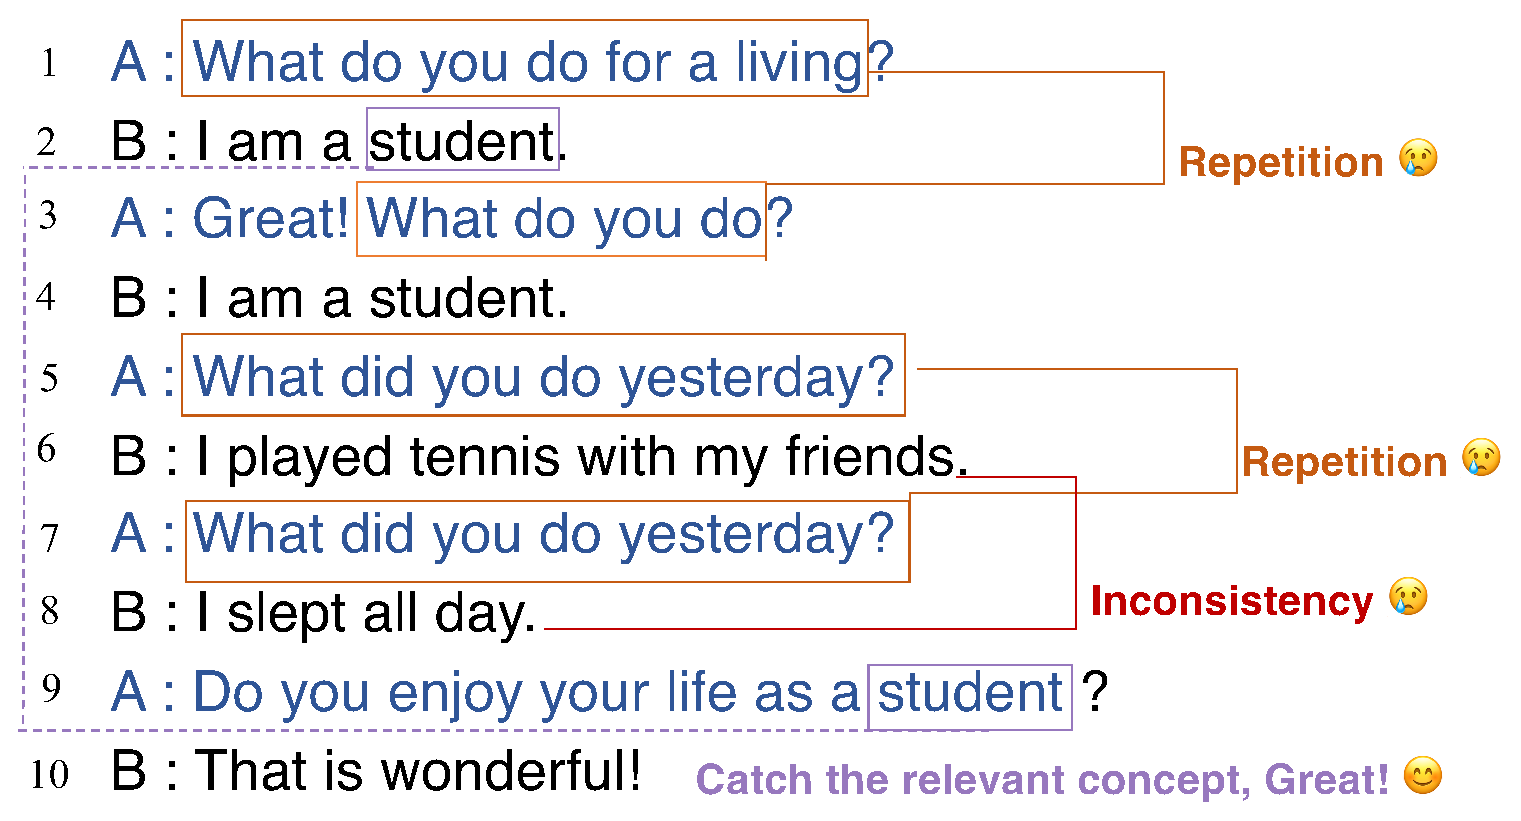
\includegraphics[width=0.95\columnwidth]{example2.eps}
        \caption{A chat snippet between two bots.}
        \label{fig:example}
\end{figure}

Fluency, Knowledge, Proactivity and Specificity are scored for each turn separately
and aggregated at the end of the conversation.
Detection for diversity, consistency and relevance are more involved and are explained
using \figref{fig:example}. 

As for diversity, at each turn $t$, we first check if there exists any repetitive question.  
We can easily find turn 3 and turn 7 repeated turn 1 and turn 5 
respectively. They will then be penalized one point for repetition. 
Repetition is not penalized if the previous turn is already 
marked as a repetitive question. For example, in \figref{fig:example}, 
although turn 4 is considered a repetition of turn 2,  
we are not going to penalize it as turn 3 is a repetitive question. 

The detection of inconsistency is always triggered after the detection of repeated questions. 
If the answers to the same questions are different, we will penalize the current turn, 
such as turn 8 in \figref{fig:example}.

We decide a repetition or an inconsistency by calculating the similarity of the two turns. 
We use a similarity function to complete the calculations, which we will 
discuss in \secref{sec:experiment}. The actual diversity and consistency scores
are the negation from the amount of repetition and inconsistency.

Relevance is assessed as a bonus to reward
a bot if it is able to memorize the important relevant concepts that have shown up 
before in the conversation. We sort the concepts that have shown up in 
chat history by their IDF scores. For example, in turn 9, $A$ 
mentions the concept word ``student'' presented by $B$ in turn 2. With this
turn, $A$ will win a bonus point.


The algorithms and notations for computing diviersty, consistency and relevance are included
in \tabref{tab:functions}, \algoref{algo:rep}, \algoref{algo:inconsist}, and \algoref{algo:bonus}. 

\begin{table}[th]
\centering
\small
\begin{tabular}{c|l}
%\hline
\toprule
\textbf{Notation} & \textbf{Description} \\ \midrule
$t$ & Current turn \\
$H(t)$  &  a list of history turns prior to $t$ \\
$Sim(x,y)$ & similarity between two turns $x$ and $y$ \\
$\sigma_r$ & Threshold for detecting repetition \\
$\sigma_c$ & Threshold for detecting consistency \\
$r$ & Weight for repetition \\
$c$ & Weight for inconsistency \\
$b$ & Weight for bonus \\
$d$ & Min distance between consecutive mentions \\
IDF list & List of lemma in chatlog sorted by IDF\\
$p$ & Percentage of important lemmas in IDF list\\
$R(t)$ &  Repetition penalty for turn $t$ \\
$C(t)$ &  Inconsistency penalty for turn $t$ \\ 
$B(t)$ &  Memory bonus for turn $t$ \\
$Rep(t)$ & A list of repeated turns for turn $t$ \\  
\bottomrule
\end{tabular}
\caption{
Functions and variables in algorithms.}
\label{tab:functions}
\end{table}

\begin{algorithm}[th]
\small
\caption{Scoring for Diversity}
\label{algo:rep}
\hspace*{0.02in} {\bf Input:}
 $t$, $H$, $Sim$, $\sigma_{r}$
; \hspace*{0.02in} {\bf Output: } 
 $R$;
\begin{algorithmic}[1]
\State //Starting to detect repetition
\For {$u$ in $H(t)$}
	\If {$Sim(t,u) \geq \sigma_{r}$}
		\State Add $u$ to $Rep(t)$
	\EndIf
\EndFor
    \If{$len(Rep(t))\geq 0$}
        \If{$t$ is a question and We can find a question in $Rep(t)$}
        \State $ R(t) \leftarrow  R(t) + 1$ 
        \Else
        \If {the previous turn of $t$ is not a repetitive question}
        \State $R(t)) \leftarrow R(t) + 1$ 
        \EndIf
        \EndIf
    \EndIf
\end{algorithmic}
\end{algorithm}


\begin{algorithm}[th]
\small
\caption{Scoring for Consistency}
\label{algo:inconsist}
\hspace*{0.02in} {\bf Input:}
$t$, $H$, $Sim$, $\sigma_{c}$
; \hspace*{0.02in} {\bf Output:  } 
 $C$;
\begin{algorithmic}[1]
\State // Inconsistency detection
 \If {previous turn of $p$ is a repetitive question} 
   \If{ the response $res$ to the question repeated by turn $p$ contradicts turn $i$ with $Sim(t, res) \leq \sigma_{c}$ }
    \State $C(t) \leftarrow C(t) + 1$
   \EndIf
  \EndIf
\end{algorithmic}
\end{algorithm}

\begin{algorithm}[th]
\small
\caption{Scoring for Relevance}
\label{algo:bonus}
\hspace*{0.02in} {\bf Input:}
$t$, $p$, $d$
; \hspace*{0.02in} {\bf Output:  } 
$B$;
\begin{algorithmic}[1]
\State // Assessing the ability of catching relevant concepts\\
$B(t) \leftarrow 0$
\For {all tokens $tk$ in current turn $t$}
 \If {$t$ - previous occurrence turn of $tk > d$ and $tk$ in the top $p\%$ of the IDF list of all tokens in the dialogue} 
   \State $B(t) \leftarrow 1$
  \EndIf
 \EndFor
\end{algorithmic}
\end{algorithm}

At the end of each game, each bot gets seven scores, one for each dimension.  
After pairwise comparison on individual dimension, a bot gains one point for win and zero point for a tie or lose.
The final score of each bot is determined by the sum of their individual scores.
%\KZ{Are these scores positive or negative? Comparable between bots?}

\subsubsection*{Match-level Scoring}
%\KZ{Use an equation to compute the final scores?}
One match which consists of two games, each started with a different bot, 
decides winning or losing between two bots.
For match-level scoring, we mimic the scoring rules of soccer tournament. 
For each match, $W$ points for the winner,  
$T$ points for a tie and 
$L$ points for the loser.
The value of $W$, $T$ and $L$ will be discussed in \secref{sec:ablation}. 

%\KZ{At the match level, we need to consider different starting context for the bots? I think we should present a few options for the reader and say that we are limited to these.}

\subsubsection*{Tournament-level Scoring}
%\KZ{Use an equation to compute the final scores?}
We count the points by simply summing up their scores gained in every match. Currently, several bots with the same final rank are tolerated. For future study, it's possible to mimic more detailed rules presented in sports match such as determine their ranking based on their win-loss relationship in the match between them.  
If they are still tied, we could propose an “overtime” for these two bots, one human judge may observe their performance and then make the decision of the game.

\section{Analysis}

We present preliminary statistical findings from ShibaScript, including lexical analysis and transcribing accuracy evaluation.
% \KZ{rewrite this preamble, it's irrelevant now: To give a detailed picture about our dataset ShibaScript and also show several statistical syntax results on it, we will explain our analysis below.}

% This is the analysis on this dataset. Inlcuding its distribution and some further analysis inlcuding bigrams.

% \subsection{Source Information}
% \label{sec:sourceinformation}
% The 16 dogs come from 16 different Japanese user accounts at YouTube. From the videos uploaded from the specific user and the captions attached to these videos, we can get to know much about the growing up environments of dogs, which will influence the expressions of these dogs to some degree. %The environments of them are in \ref{tab:sourceinformation}.
%这是狗的来源的信息,包含地区、是否家养、之类的

% \begin{table}[th]
% \centering
% \begin{tabular}{c|c|c|c}
% \hline
% \textbf{Dog Index} & \textbf{Color} & \textbf{Other Pets} & \textbf{Area}\\\hline
% 0 & yellow & \\
% 1 & yellow & \\
% 2 & yellow & \\
% 3 & yellow & \\
% 4 & yellow & \\
% 5 & yellow & \\
% 6 & yellow & \\
% 7 & yellow & \\
% 8 & yellow & \\
% 9 & yellow & True \\
% 10 & yellow & \\
% 11 & yellow & \\
% 12 & yellow & \\
% 13 & yellow & \\
% 14 & yellow & \\
% 15 & black & \\\hline
% \end{tabular}
% \caption{The source information of dogs in ShibaScript. Color means the fur color of the dog. Other Pets means whether the dog is kept with a family with other animals. Area means the living locations of the family.}
% \label{tab:sourceinformation}
% \end{table}



% \begin{table}
% \centering
% \begin{tabular}{c|c|c|c|c}
% \hline
% \multirow{2}{*}{\textbf{DogID}} & \multicolumn{2}{c|}{\textbf{Sentence}} & \multicolumn{2}{c}{\textbf{Word}}  \\
% \cline{2-5}
% {} & \textbf{Num} & \textbf{Length(s)} & \textbf{Num} & \textbf{Length(s)} \\
% \cline{1-5}
% 0 & 346 & 1107.67 & 577 & 363.36\\
% 1 &  158 & 514.24 & 241 & 129.00\\
% 2 & 553 & 1643.00 & 847 & 469.20\\
% 3 &  55 & 171.69 & 123 & 65.52\\
% 4 & 56 & 224.00 & 107 & 94.08\\
% 5 &  115 & 374.58 & 217 & 98.52\\
% 6 & 52 & 157.00 & 77 & 47.72\\
% 7 & 40 & 135.00 & 65 & 27.44\\
% 8 &  135 & 566.03 & 316 & 143.68\\
% 9 & 255 & 795.00 & 408 & 157.08\\
% 10 & 1188 & 4306.00 & 2029 & 1372.52\\
% 11& 188 & 570.94 & 320 & 203.20\\
% 12  & 130 & 562.28 & 257 & 147.00\\
% 13  & 993 & 2930.19 & 1719 & 749.72\\
% 14  & 118 & 350.11 & 324 & 144.76\\
% 15  & 87 & 299.88 & 134 & 101.24 \\\hline
% sum & \textbf{4469} & \textbf{14707.61} & 7761 & 4314.04\\\hline
% \end{tabular}
% \caption{The basic statistical information of ShibaScript.}
% \label{tab:datasetinformation}
% \end{table}




\subsection{Lexical Analysis}
During the transcribing, there are in total 11 types of tokens, in which 9 types are phonetic symbols~(\tabref{tab:alphabet}), the other two are short pauses between words and long pauses between sentences. 

Similar to humans, the length of these tokens contain ample information. The exact lengths of tokens are kept in ShibaScript for concrete analysis. Because the long pauses are largely determined by the scene at that time, the numerical analysis of it will not be included here. 


\begin{table}[th]
\centering
\small
\begin{tabular}{c|c|c}
\hline
\textbf{Symbol} & \textbf{Mean len (s)} & \textbf{Variance (s)}\\
\hline
\verb|[au]| & 0.35 & 0.022 \\
\verb|[a]| & 0.35 & 0.017 \\
\verb|[^]| & 0.34 & 0.017\\
\verb|[u:]| & 0.45 & 0.054\\
\verb|[u]| & 0.35 & 0.030\\
\verb|[i]| & 0.33 & 0.020\\
\verb|[k]| &  0.24 & 0.009\\
\verb|[(w)au]| & 0.34 & 0.018\\
\verb|[en]| & 0.36 & 0.032\\
\verb|short pause| & 0.57 & 0.335\\
\hline
\end{tabular}
\caption{The mean and variance of the duration of 9 phonetic symbols 
and short pauses between words.}
\label{tab:tokenanalysis}
\end{table}

The mean and variance of each token length can be seen in~\tabref{tab:tokenanalysis}. In which we find that almost every phonetic symbol has a similar length of 0.35s or so. Except for the phonetic symbol \verb|[u:]|, which is a prolonged sound owning an average length of 0.45s. While phonetic symbol \verb|[k]| is a relatively short-lived symbol, only having 0.24s average length.

Considering the monogram~(\figref{fig:monogram}) of ShibaScript, we can find that the most frequent symbol is \verb|[en]|, which reaches to 3478 times in ShibaScript, the following two are \verb|[au]| and \verb|[a]|, which reaches  1981 and 2011 times respectively. One of the reasons why \verb|[en]| exceeds much, which is counterintuitive, is that symbols such as \verb|[a]|, \verb|[au]|, \verb|[(w)au]| are divided up. The least frequent symbol is \verb|[k]|, which only reaches 15 times. This is because dogs seldom produce air-sounds like \verb|[k]|.

At the same time, we can find that these phonetic symbols exist in multiple dogs' sounds, showing that these 9 symbols are universal.

\begin{figure}[th]
\centering
\scalebox{0.32}{\includegraphics{monogram.pdf}}
\caption{The occurrences of each monogram. The blue bars show the occurrences across the whole dataset of each monogram in ShibaScript, the green lines show the numbers of dogs producing the symbols, from 1 to 16.}%\KZ{Remove ``Monogram Stats'' from the pic, since
% you already talk about it in the caption.}
\label{fig:monogram}
\end{figure}

%静音片段分析
%unigram, bigram分析
After analyzing the monogram, we come to find the relationship between symbols, as well as the bigram~(\figref{fig:bigram}) of ShibaScript. Among these bigrams, several appear extremely frequently. It shows a possibility that they are associated with some common semantic meanings. We will dive into that in the future works. Due to space constraints, the detailed information of bigram is shown in~\secref{sec:appendixc}.

% 1 
\begin{figure}[th]
\centering
\scalebox{0.32}{\includegraphics{bigram.pdf}}
\caption{The occurrences of each bigram. The blue bars show the occurrences across the whole dataset of each monogram in ShibaScript, the green lines show the numbers of dogs producing the symbols, from 1 to 16.}
\label{fig:bigram}
\end{figure}




\subsection{Accuracy of Transcription}
In this paper, we discover the certain phonetic pattern of Shiba Inu dogs and assign a vocal dictionary of 9 symbols, which is a first-step trial in this area. To better evaluate the phonetic symbols set as well as the integral accuracy of our transcribing, we have done an evaluation test on these two aspects. The evaluation metric is 5-level Mean Opinion Score~\cite{viswanathan2005measuring}. Three raters will give scores to either one syllable or one word according to~\tabref{tab:ratestandard}. %\MY{How many raters?}


\begin{table}[th]
\centering
\small
\begin{tabular}{c|l}
\hline
\textbf{Score} & \textbf{Description} \\
\hline
5 & The label exactly matches up.\\
4 & Some difference exists between the\\
{}& label and the sound. Humans are s- \\
  & ometimes hard to distinguish.\\
3 & Difference exists between the label\\
  & and the sound. Humans can tell the \\
  & difference immediately.\\
2 & Although the label is obviously wr-\\
{}& ong, there is similarity between t-\\
{}& he label and the sound.\\
1 & The label is totally wrong. \\
% 5 - Excellent 完全一致,失真程度不可察觉
% 4 - Good 有轻微不一致,失真程度略可察觉,如a和ao, u和u:,(w)au 和au,人耳有时也会难以分辨其中差异
% 3 - Fair 一般,失真程度可察觉,人耳可以轻松分辨出二者差异
% 2 - Poor 差,失真程度尚可接受,可以找到一丝相似
% 1 - Bad 很差,失真程度难以接受, 完全不同
\hline
\end{tabular}
\caption{The evaluation metric of rating, which is similar to MOS in speech synthesis evaluation metric.}
\label{tab:ratestandard}
\end{table}

\subsubsection{Phonetic Symbol Accuracy Evaluation}
\label{sec:phone_eva}
%在音素层面进行的evaluation
For each syllable category, we select 50 syllables randomly. The rating result is in~\figref{fig:phoneticaccuracy}. The Fleiss Kappa~\cite{kilicc2015kappa} between three annotators is 0.609.

\begin{figure}[th]
\centering
\scalebox{0.30}{\includegraphics{phoneticaccuracy.pdf}}
\caption{The evaluation result of 9 phonetic symbols. }
\label{fig:phoneticaccuracy}
\end{figure}

% \KZ{Fonts too small, and the image is not clear. Every image must be critical clear after ampification. Use vector images (not bitmap) whenever possible.}

\subsubsection{Word Accuracy Evaluation}
%在word层面进行的evaluation
For the word accuracy evaluation, we select 30 words for each dog randomly and find the same person who rates for phonetic symbols to score for them. The rating result is in~\figref{fig:wordaccuracy}. The Fleiss Kappa between three annotators is 0.516.

\begin{figure}[th]
\centering
\scalebox{0.29}{\includegraphics{wordaccuracy.pdf}}
\caption{The evaluation result of words for 16 different dogs.}
\label{fig:wordaccuracy}
\end{figure}

\section{Evaluation}
\label{sec:exper}


In this section, we discuss the experiment design and experiment
 result analysis for the proposed watermarking technique.

\subsection{The Experimental Setup}
We will implement the partitioning, watermark inserting,
and watermark detecting algorithms and observe the performance 
of our proposed algorithms under different potential attacks.
Both algorithms have been implemented with C and all
experiments were conducted on Core PC with 2.0 GHz
CPU and 2 GBytes of memory running the Ubuntu 12.04 operating system.
All editing operations on the digital road maps in Shapefile are
accomplished by SAGA software \cite{sagaurl}. 

\begin{figure}[ht]
\centering
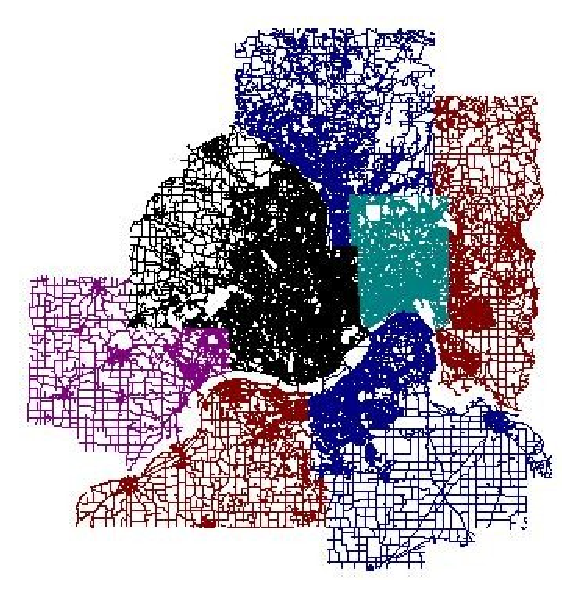
\epsfig{file=region.eps,width=0.5\columnwidth}
\caption{Twin-Cities Seven-County Road Map}
\label{fig:region}
\end{figure}


\subsubsection{GIS Spatial Data Set}

We use the Minnesota (MN) state base map of the Minneapolis-St. Paul 
Metropolitan area as our GIS spatial data set to analyse the performance 
of our proposed watermark algorithm. More specifically we use MN state base 
map of seven counties, namely, Anoka, Carver, Dakota, Hennepin, Ramsey, Scott, 
Washington, as our real dataset for this experiment. 
This base map we select is in ShapeFile format\cite{shapefileurl}, 
specifically in the Measured Polyline 
type. In this dataset, there are in total 415,651 line segments
and 372,466 different points. Figure \ref{fig:region} shows the visual map
of digital data for these seven counties. This data set can
be downloaded from the MN/DOT web site\cite{mndoturl}. Since the data
set is in the ShapeFile format originally, we need first to
transform it into text format and manipulate this text file in our algorithm.


\subsubsection{Experiment Design}

The purpose of this experiment is to analyse the performance of our proposed 
watermark approach under different attack scenarios. An original GIS spatial 
data set, watermarks, and secret keys are fed into the watermark insertion 
module and watermarked GIS spatial data is output. Then this watermarked data 
set is attacked by different possible attacks that are differentiated by 
different attack parameters. Finally, the attacked watermarked data and the 
secret keys used in the watermark insertion module are input into the watermark 
detection module to extract the inserted watermarks that will be used to check 
whether the GIS spatial data set has been used illegally.


%\KZ{%Say clearly how you obtain the cropped and merged and noise test data set.
%Show some example snapshot if possible.\\
%For each original map, one watermarking scheme and one attack method,
%there are basically three things we need to measure:\\
%1) amount of distortion added by the watermarking;\\
%2) detection accuracy;\\
%3) execution time for insertion and for detection\\
%With the about result data, we can probably design various ways to showcase it, e.g.,
%average over different maps, or a scatter plot of times, or correlation plot between
%distortion and accuracy, etc.
%}

In order to evaluate the robustness of our watermarking algorithms (which is called
Jiang in the rest of this section), we illustrate 
the performance of our proposed watermark approach under different attacks with 
different settings. In this part, we compare the proposed approach with two other 
watermarking algorithms proposed by Pu\cite{PuDJ06} and 
Voigt\cite{Vogit:2003}. Both methods are blind watermarking algorithms and provide 
some resistance to crop attack. We control the accuracy lost of the experiment data 
caused by different methods and compare the performance of them under noise attack, 
crop attack and merge attack. In this section, ``crop ratio'' and ``merge ratio'' 
means the area ratio we crop from the total watermarked map.

\subsection{Performance under Noise Attack}
Attackers will randomly select subsets of watermarked map to add noise. Meanwhile, to 
keep the usability of the map, those subsets could not take too much parts of the total 
map. In this experiment, we watermark the map of St. Paul area and attack the watermarked 
map with some random Noise, perturbing the map with different accuracy lost. 

In this noise attack experiment, we watermark the map with three algorithms in certain 
distortion. After that we attack the watermarked maps with different noise distortion. 
For each noise distortion, the noise will be added in different methods for 20 times. 
For all three methods, the noise added is ``exactly'' the same each time.
At last, we detect the watermark and calculate detection accuracy for three algorithms. 
We set distortion $\delta_w$ added by the watermarking as $10.5\times 10^{ -6 }$ (Jiang), 
$10.8\times 10^{-6}$ (Voigt) and $9.8\times 10^{-6}$ (Pu). Take the size of map into consideration,
these distortion can be deemed at the same level. On the other hand, the noise distortion 
$\delta_n$ is changed from $5.12 \times 10^{-3}$ to 
$2.56 \times 10^{-2}$. Actually, $\delta_n$ here is large enough that almost changes all 
vertexes of the map. Figure \ref{fig:noise} shows the results.
%\KZ{%Does it make sense to have different distortion levels for three
%experiments? 
%I think we want to compare the trend against $\delta$ for
%these three experiment to show that our method is less sensitive to distortions.
%Also I think we want graphs/tables that show how performance varies with
%different $\delta$ (noise) and different $\delta$ (watermarks). These two
%$\delta$'s are different but it will be good if we can show both in one graph.}
%\KZ{It's called ``distortion'', not ``distortion distance'', because 
%it's measured globally for the whole map and not for each individual points.
%Are you going to apply the noise to only subset of the points or 
%all the points?
%In any case, you need to make sure you apply the *exactly* the same distortion
%(i.e., same distortion at the same point) to the map for each of the 3 methods, though 
%the watermarks for these 3 methods maybe different.}
 


\begin{figure}[th]
\centering
\epsfig{file=noiseattack.eps,width=0.7\columnwidth}
\caption{Performance under Noise Attack %\KZ{Why is Voigt almost the same
%as us? Why is Yu-Chi so bad? Btw, it should be Yu-Chi, not Yuchi in all
%the graphs.}
}
\label{fig:noise}
\end{figure}

In this experiment, we set the standard of positive detection as correctly
decide the whole map is watermarked. However, in fact, according to the 
detection method of our algorithm, some more assistance can be obtained.
Even the whole map is failed to be detected, the result could be a series
of subregions that is suspicious. 
The results shows that our algorithm successfully survived noise 
attack. On one hand, we watermark certain bits which will not be directly affected by 
the noise if perturbing for individual vertex is under certain strength. 
Meanwhile, even the perturbing for individual vertex is powerful enough, 
$\theta $ and the hash function of $sl$ in in partition and insertion 
algorithms provide a good tolerance for it. 
   
\subsection{Performance under Crop Attack}
%\JK{For crop attack, I plan to implement three experiments.\\ 
%1). Watermark a map in certain strength and crop it into seven county 
%maps. Then I will give a table of detection confidence of each cropped 
%map. \\ 
%2). I will watermark the map with different distortion distance, and then 
%crop them to a certian ratio, e.g. 1/2, for 20 times. Then the result 
%will be a ``detection accuracy-distortion'' figure. In this experiment,
%a ``time-distortion'' figure can also be obtained.\\
%3). From the 2) experiment, we select the minimum ``distance'' to watermark
%a map, then crop it in different ratio. For each ratio, 20 different cropped
%maps will be detected. The result will be a ``Detection accuracy-crop ratio'' 
%figure for all three algorithms. }
%\KZ{%How do you crop into 7 maps, one for each county? I thought you use
%an automatic way of cropping now which means you can only crop out rectangular
%maps? 

%For (2) it can be a scatter plot, x-axis been distortion, y-axis being
%detection accuracy. The time-distortion can also be scatter plot (see Zhixian's
%paper for an example) Also for (2) you can have one plot for each algo, or
%plot all three together together on one plot but using different color or 
%different point styles. For (3) I don't understand what you mean by
%minimum ``distance''. But I sort of see the meaning of detection accuracy
%vs. crop ratio. This experiment shows how strong we are in ``massive crop''
%attacks, right? I think all 3 experiments are good!}

In our experiment, on one hand, each county out of seven is selected to be 
detected. On the other hand, some certain proportion of the map is selected 
to evaluate the performance of our algorithm. 

In this experiment, the parameter $\theta $ is set as 30,000.0 
($\delta_w=10.5\times 10^{ -6 }$) and the square side 
length is 100.0 for both insertion and detection. We partition the whole map 
of Minneapolis-St. Paul Metropolitan area. Then the watermarked map is split 
according to the boundary of different counties. After that, we impose our 
watermarking algorithm on these ``partial'' maps, trying to decide whether the 
maps are parts of our original map. Table \ref{tab:crop} shows the results of 
this experiment. 

\begin{table}[ht]
\centering
\caption{Crop Attack Detection}
\label{tab:crop}
\begin{tabular}{|c||c|c|c|c|} 
\hline
County & Total & Match & Confidence & Result \\\hline \hline
Anoka & 55 & 51 & 1.000 & positive\\\hline
Carver & 28 & 23 & 0.999 & positive\\\hline
Dakota & 68 & 61 & 1.000 & positive\\\hline
Hennipin & 141 & 137 & 1.000 & positive\\\hline
Ramsey & 58 & 56 & 1.000 & positive\\\hline
Scott & 29 & 25 & 0.999 & positive\\\hline
Washington & 46 & 43 & 1.000 & positive\\\hline
\end{tabular}
\end{table}

By analysing the insertion algorithm, we can easily get the notion that the 
partition criterion $\theta $ has a large influence on the result of our watermark 
algorithm. We also design a series of experiments to figure out the influence 
of the $\theta $. In this experiment, we watermark the map with different distortion 
(\ref{equ:distort}) by adjusting $\theta $ (see Figure \ref{fig:dis}) and then select 
the crop ratio of $1/2$, $1/4$ and $1/8$ of the map to detect. Each ratio is detected 
for 20 times.  Figure \ref{fig:m} show the result of experiments. 
Insertion (Figure \ref{fig:ti}) and detection (Figure \ref{fig:td}) time 
for different distortion is also measured.

\begin{figure}[th]
\centering
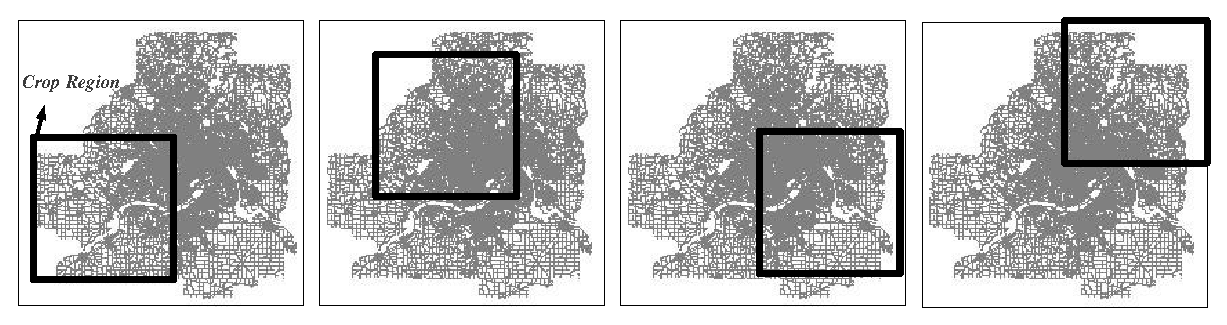
\epsfig{file=cropmethod.eps,width=\columnwidth}
\caption{A Showcase of Crop Ratio 1/4}
\label{fig:cropmethod}
\end{figure}

%\begin{figure}[th]
%\centering
%\epsfig{file=mparameter.eps,width=0.8\columnwidth}
%\caption{Performance Under Different Distortion}
%\label{fig:m}
%\end{figure}

%\begin{figure}[h]
%\centering
%\epsfig{file=mdelta.eps,width=0.6\columnwidth}
%\caption{Distortion Added by Watermarking}
%\label{fig:dis}
%\end{figure}

\begin{figure}[th]
\centering
\subfigure[Distortion]{
  \label{fig:dis}
  \epsfig{file=mdelta.eps,width=0.45\columnwidth}
}
\subfigure[Different Crop Ratio]{
  \label{fig:m}
  \epsfig{file=mparameter.eps,width=0.45\columnwidth}
}
\subfigure[Time of Insertion]{
  \label{fig:ti}
  \epsfig{file=time.eps,width=0.45\columnwidth}
}
\subfigure[Time of Detection]{
  \label{fig:td}
  \epsfig{file=time1.eps,width=0.45\columnwidth}
}
\caption{Experiment Results Under Different Distortion}
\label{fig:pudd}
\end{figure}

%\begin{table}[th]
%\centering
%\caption{Distortion Added by Watermarking}
%\label{tab:dis}
%\begin{tabular}{|c||c|c|c|c|c|c|c|c|} 
%\hline
%$\theta$(km) & 3 & 5 & 10 & 15 & 20 & 25 & 30 & 35 \\\hline \hline
%$\delta (10^{-6})$ & 10.50 & 6.60 & 3.05 & 2.00 & 1.84 & 1.33 & 1.09 & 0.94 \\\hline
%\end{tabular}
%\end{table}

In the following experiment, we watermark a map with certain distortion, here we set 
$\theta =30,000$. After that we crop different ratio from the map to evaluate the performance 
of our algorithm. For each crop ratio, we select different parts of the map to detect 
up to 20 times. We randomly select different parts of the watermarked map to detect (see 
Figure \ref{fig:cropmethod}) and calculate the detection accuracy. Here we also implement 
Voigt's and Pu's methods to make a comparison. Distortion $\delta_w$ added by the watermarking 
is $10.5\times 10^{ -6 }$ (Jiang), $10.8\times 10^{-6}$ (Voigt) and $9.8\times 10^{-6}$ (Pu). 
The distortion of all three methods are almost at the same level.
Figure \ref{fig:cropattack} gives the results.

%\begin{figure}[th]
%\centering
%\subfigure[Time of Insertion]{
%  \label{fig:ti}
%  \epsfig{file=time.eps,width=0.45\columnwidth}
%}
%\subfigure[Time of Detection]{
%  \label{fig:td}
%  \epsfig{file=time1.eps,width=0.45\columnwidth}
%}
%\caption{Experimental Time Results}
%\label{fig:results}
%\end{figure}

\begin{figure}[th]
\centering
\epsfig{file=cropattack.eps,width=0.7\columnwidth}
\caption{Performance Under Different Crop Ratio}
\label{fig:cropattack}
\end{figure}

According to the experiment result, we can find that our algorithm keeps a perfect
result when the crop ratio is up to $1/8$, while the comparison methods show a significant
accuracy degradation. And when crop ratio is $1/16$, we still contain a high accuracy.
We also test the detection accuracy under different distortion in $1/8$ crop ratio
(see Figure \ref{fig:mdelta}). In this experiment, our algorithm can attain
a $100\%$ detection accuracy with just little distortion. Since the detection accuracy of 
our algorithm quickly attain to $1$, it is not necessary to plot too many points in Figure 
\ref{fig:mdelta}.

\begin{figure}[h]
\centering
\epsfig{file=delta.eps,width=0.7\columnwidth}
\caption{Detection Accuracy in $1/8$ crop ratio}
\label{fig:mdelta}
\end{figure}

\subsection{Performance Under Merge Attack}
%\JK{For merge part, I plan to design two experiments:\\
%1).I plan to watermark a map with the same distortion distance as crop 3) and 
%make a merge map like figure \ref{fig:merge}. What I want to show the readers is
%a direct result of the merge detection result: suspicious regions and detection
%confidence. A visual figure can also be drawn.\\
%2).Just like merge 3), I plan to crop the watermarked map into different ratio
%and merge with the other data source to make different maps, for each ratio, 20
%different merge maps will be detected. The result will be a ``Detection accuracy-
%watermarked ratio''figure for all three algorithms.} 

%\KZ{So (1) is a special case of (2) which is actually fig 15 right? For
%(1) you will just have a detection number for 3 algorithms? I think you can
%show visually what was the original merge situation and what was the 
%portion that you detected by comparing and contrasting the difference in
%a figure. That will be visually impactful.}

In this experiment, we select the $2012$ TIGER map of Minneapolis-St. Paul 
Metropolitan area as another data source, which can be downloaded from the 
United States Census Website\cite{tigerurl}. The coordinate system of TIGER 
map is different from MN dot base Map. We transform the coordinate system of 
TIGER map to make it same as the former data source. Figure \ref{fig:17} is 
the overlap of these two maps of Anoka county after the synchronization. 
As we can see that very slight difference could be found between these two maps, 
so we have a good reason to believe that if we implement our partition algorithm 
on a merge map of them, the result will almost be the same.


\begin{figure}[th]
\centering
\epsfig{file=overlap.eps,width=0.8\columnwidth}
\caption{Overlap of Two Maps}
\label{fig:17}
\end{figure}
We crop a watermarked map ($\delta_w = 6.60 \times 10^{-6}$) and merge part of it with TIGER 
map to make a ``new'' map (see Figure \ref{fig:mergeexp1} (a)). The result of the 
merge detection: suspicious regions and detection confidence is shown in Table 
\ref{tab:merge}. Here we select those regions which have at least 10 points tested. 
From the corresponding visual figure (see Figure \ref{fig:mergeexp1} (b)), we can see 
that our algorithm almost ``exactly'' decides the suspicious regions. 

\begin{figure}[th]
\centering
\epsfig{file=merge.eps,width=0.9\columnwidth}
\caption{Merged Map}
\label{fig:mergeexp1}
\end{figure}


\begin{table}[th]
\centering
\caption{Merge Attack Detection}
\label{tab:merge}
\begin{tabular}{|c||c|c|c|c|} 
\hline
Region & Total & Match & Confidence & Result \\\hline \hline
1 & 147 & 122 & 1.000 & positive\\\hline
2 & 12 & 11 & 0.997 & positive\\\hline
3 & 23 & 18 & 0.994 & positive\\\hline
4 & 15 & 12 & 0.983 & positive\\\hline
\end{tabular}
\end{table}

We also watermark the Minneapolis-St. Paul Metropolitan area and then split this 
watermarked map into the same small portions as cropping experiment above. After 
that we merge these maps with the complementary parts of map from TIGER to create 
some new digital road maps. In this experiment, we also implement the two other 
method to make a comparison. Distortion $\delta_w$ added by the watermarking still
is $10.5\times 10^{ -6 }$ (Jiang), $10.8\times 10^{-6}$ (Voigt) and $9.8\times 10^{-6}$ (Pu). 
Figure \ref{fig:mergeattack} shows the result of our 
experiments.
\begin{figure}[th]
\centering
\epsfig{file=mergeattack.eps,width=0.8\columnwidth}
\caption{Performance Under Merge Attack}
\label{fig:mergeattack}
\end{figure}

Comparing with the cropping experiment, we can obviously find the performance of 
our proposed algorithm is almost not affected by the complementary part of the map. 
However, the detection accuracy of the other two methods decrease significantly. 
The reason is the complementary map provides sufficient disturb to watermarked data.
Similarly, we also implement another experiment to evaluate the relationship between
detection accuracy and watermark distortion $\delta_w$. From this figure, we can see that
our algorithm still can quickly attain a quite high detection accuracy. However, when 
$\delta_w$ increases for Pu's and Voigt's method, the detection accuracy doesn't changed significantly.
The reason for Pu should be that it's global liner correlation is destroyed by ``merge'' attack.
For Voigt's method, though more watermark information is used for detection, more ``merge'' 
noise will will also be added to the detection process. Thus increase of detection accuracy
for them is not significant.



\begin{figure}[h]
\centering
\epsfig{file=deltamerge.eps,width=0.7\columnwidth}
\caption{Detection Accuracy in $1/8$ Merge ratio}
\label{fig:deltamerge}
\end{figure}



\subsection{Analysis}

As is illustrated in the experiments above, to preform well in detection parts, 
the selection of parameter $\theta$ is significant. If $\theta$ is smaller, the partition
step will construct a larger quadtree, which means we will make more distortion
 into the map. In this case, the result of detection we get will be more accuracy,
but at the same time, the partition process will be more time-consuming. However, $\theta$
is a measurement of road length, it varies from different maps. It is impossible to
set a uniform standard for $\theta $. In our algorithm, another information related to 
$\theta$ is the number of leaf nodes of the corresponding quadtree N. So we could discuss
N instead. Anytime detecting a suspicious map, no matter a complete one or just a part, 
we have to guarantee the accuracy of detection. In other words, partition of the 
suspicious map should output enough subregions. To resell the digital map, an attack 
should firstly keep the usability of the map not only in accuracy degradation but
also in size of the map. For example, if the map of Minnesota state is watermarked
and published. An attacker who want to resell part of this map may prefer to crop a 
sub-map of a county from the whole map. Thus the partition algorithm should partition 
a county map into enough subregions, which can guarantee the accuracy of detection according 
to the probability formula \ref{pe}.



%%% Local Variables:
%%% mode: latex
%%% TeX-master: "paper"
%%% End:

\section{Related Works}
\label{sec:relate}

Most existing related works just consider the contact history but do not consider the map information. \cite{Whitbeck10:Plausible} solve this problem by force analysis. It assumes that there exists four different forces as attraction, repulsion, drag and anticipated attraction, furthermore each node will be affected by these four forces at any moment. This paper take each contact history as the anticipated attraction, then through force analysis they infer the traces out to get the map information. But in the real world, we can't justify there really exist such kinds of forces. Even though these forces really exist, but we wonder whether these forces could lead to the node's movement.  

Some other works \cite{Vtrack} \cite{Malnet} \cite{Vulnerability} could infer the trace by GPS information which is actually not available in 
our work.

\section{Conclusion}
\label{sec:conclude}
In this work,
we propose a new data creation method to generate
 a semi-structured synthetic training data for 
opinion summarization,
which is known for lacking training data.
\cut{We showed that by extracting an aspect-opinion pairs and 
implicit sentences from multiple reviews
first and then synthesizing them into semi-structured data, we achieve
better performance on opinion summarization.}
%\KZ{It is critical to show in your experiments that the proposed
%synthetic data is better than other possible alternatives.}, 
We also designed an aspect-guided model with opinion-aspect pair encoder and implicit sentence encoder.
The results showed that
the proposed model can make full use of semi-structured data
and generate high-quality summaries.





\bibliographystyle{abbrv}
%\renewcommand{\baselinestretch}{0.9}
\bibliography{watermark}
% watermark.bib is the name of the Bibliography in this case
\end{document}
